\chapter{Concept}
\label{ch:concept}
This chapter presents the theoretical concept of WebArgo as a foundation for the following chapters. The first section defines the terminology used to describe the various actors and entities of WebArgo. Following this, the next section presents WebArgo's architectural design and its key components. The last section of this chapter introduces the underlying theoretical model of WebArgo, which describes the constraints and conditions necessary to achieve potential performance improvement by utilizing the WebArgo platform.

\section{Terminology}
\label{sec:concept:terminology}
This section defines the fundamental terms used to describe all entities and actors of WebArgo. These precise definitions establish all terms used to describe WebArgo's processes in the following chapters of this work.

\subsection{Job}
\label{subsec:concept:job}
A job represents a computational problem or project to be processed or solved by participating volunteers of WebArgo. Jobs are required to be parallelizable, hence a job can be divided into multiple tasks for parallel execution of tasks.

\subsection{Task}
\label{subsec:concept:task}
Each job is divided into multiple tasks and ideally has each task an equal computational workload. Therefore, each task represent a unique, atomic unit of computational workload from its assigned job. Additionally, each task is required to operate independently and therefore requires no communication to other tasks during execution. These tasks are distributed among the volunteer participants of WebArgo to achieve parallel processing of the entire job.

\subsubsection{Batch}
\label{ssubsec:concept:batch}
A batch is defined to be a subset of tasks, wich are all assigned to the same job.

\subsubsection{Worker}
\label{subsec:concept:worker}
Workers are volunteers who contribute the computational resources of their consumer device to participate in WebArgo and therfore support jobs computed by the WebArgo platform. They receive tasks from the current batch, compute them using their local resources, and transmit the task results to the WebArgo platform.

\subsubsection{Administrator}
\label{ssubsec:concept:admin}
Administrators manage the WebArgo platform. Therefore, they have the ability to control job execution, monitor overall job progress and monitor the connected workers. Additinally, administrators can develop custom jobs to distribute their project through the WebArgo platform.

\subsection{Backend}
\label{subsec:concept:backend}
The backend is used as the central component to maintain the network. Each client (worker \& administrator) intending to connect to WebCrowd must establish a WebSocket connection to the backend. Additionally, the backend is responsible for scheduling and distributing the tasks of a job among all participating workers. Furthermore, the backend is responsible to manage information about all jobs and to persistently store the results of all completed tasks.

\subsection{Frontend}
\label{subsec:concept:frontend}
The frontend enables the connection between workers or administrators and the backend. Furthermore, it represents a interactive \ac{UI} for the connected clients and is responsible to provide the WebAssembly environment for the workers.

\section{Architecture}
\label{sec:concept:architecture}
The WebArgo platform consists of the following three components:
\begin{itemize}
    \item Backend (\autoref{subsec:concept:backend}) handling the distribution of tasks
    \item Frontend (\autoref{subsec:concept:frontend}) providing the interface of the web application for all clients
    \item Database used to persist job and job progress data
\end{itemize}
\autoref{fig:concept:architecture} illustrates the architecture of WebArgo. The web server that hosts the WebArgo platform serves the backend and the frontend on independent ports. Any heterogenous clients, diverse in hardware and operating system, are able to connect to WebArgo, if they use a web browser that supports WebAssembly, WebSockets and WebWorker. These clients access the platform by connecting to the frontend, which than establishes the WebSocket communication between the client and the backend. Each client (worker \& administrator) always maintains a bidirectional WebSocket connection to the backend. The database is used to persistently store data about jobs and the progress of each job, and is exclusively accessible by the backend.
\begin{figure}[htbp]
    \centering
    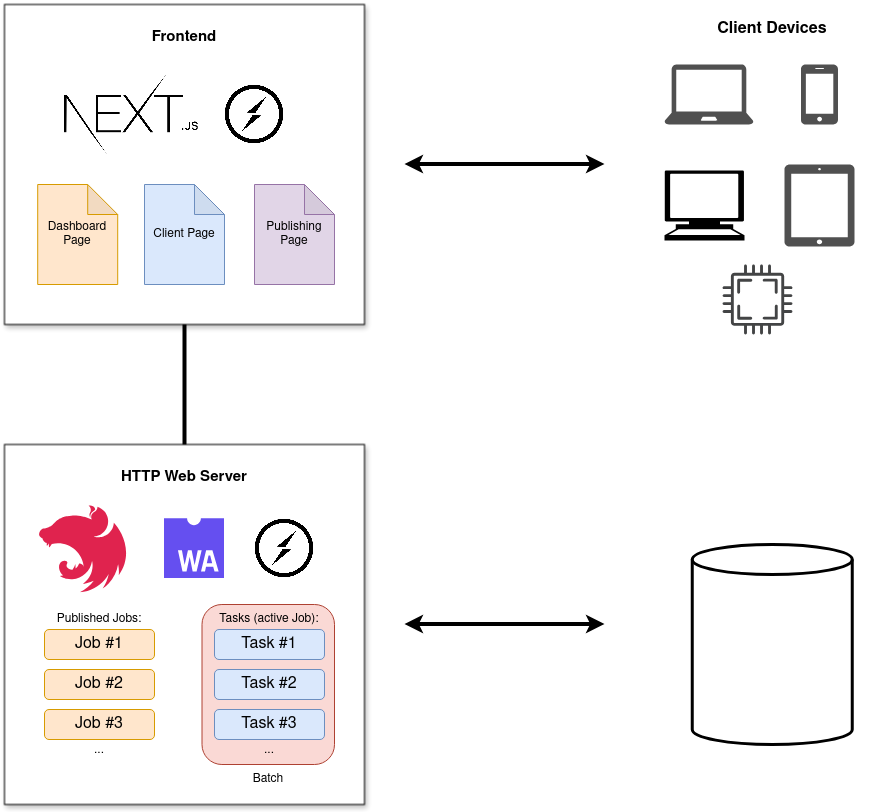
\includegraphics[width=0.95\textwidth]{gfx/figures/WebAssembly-MA.png}
    \caption{Architecture Modell of the Platform}
    \label{fig:concept:architecture}
\end{figure}

\section{Theory}
\label{sec:concept:theory}
(TODO) Include Amduls law 

This following section displays the mathematical and theoretical background of the developed volunteer computing network. The objective is to identify the constraints that must be satisfied to ensure that the use of a volunteer computing network offers advantages over regular local computing on a single device.

The primary constraint is that the program code, which is distributed across multiple devices, must be capable of parallel execution. This allows all participating devices to each compute a portion of the overall workload simultaneously. In this context, a parallelizable job is characterized by the following properties:
\begin{itemize}
  \item The problem can be divided into multiple tasks.
  \item Each task executes the same program code.
  \item Each task can receive specific input parameters to process a distinct part of the problem.
  \item Each task operates independently, with no need for communication between tasks and no dependencies to other sequentially preceding tasks.
\end{itemize}
The total estimated execution time of a problem that is divided into \emph{T} tasks which are computing an equal amount of workload and are executed sequentially is denoted as $t_{ExSeq}$. It is assumed that, on average, each of these tasks requires a computing time of $t_{Native}$ when executed in the native environment. Consequently, the total computation time for the sequential execution of a problem on a single device is expressed as:
\begin{equation}
  t_{ExSeq} = T \cdot t_{Native}
  \label{equ:single}
\end{equation}
When \emph{T} equal tasks are distributed over \emph{N} independent nodes, the total computation time is expected to be proportionally reduced, because the workload is being parallelized. This reducing factor \emph{I} represents the amount of iterations needed to distribute all tasks \emph{T} over \emph{N} nodes and is described by the fraction of \emph{T} divided by \emph{N}. Since \emph{T} and \emph{N} are part of the natural numbers $\mathbb{N}$ and a single task can not be split into smaller chunks, \emph{I} is also part of the natural numbers $\mathbb{N}$. In order to esure that the result of the devision is always a natural number the Gaussian ceiling function is applied here. Hence, \emph{I} is given by: 
\begin{equation}
  I = \bigg\lceil\frac{T}{N}\bigg\rceil
  \label{equ:frac}
\end{equation}
(TODO) Change calculation from latency to overhead = latency + file Size input \& wasm + gluecode (?) + (latency) + file size result
(TODO) replacy latency for overhead and use latency in calculation

Furthermore, when a problem is distributed across \emph{N} nodes over a network connection, the network latency must be taken into account in the computation of the total execution time $t_{ExDist}$. The latency, denoted as $t_{L}$, consists of the time required to send input arguments to a single device and the time needed to receive the result from a single task. It is assumed that the program code necessary to execute a task is loaded on all devices in advance, and therefore, the initial overhead of this process is excluded from the calculation. 
(TODO) overhead estimate calculation

Additionally, it is assumed that the computation time $t_{Virtual}$ of each task executed in the virtualized environment is equally long across all independent nodes \emph{N}. Thus, the total execution time $t_{ExDist}$ for a parallelizable problem distributed across \emph{N} nodes can be expressed as:
\begin{alignat}{4}
  t_{ExDist} &= I \cdot (t_{Virtual} + t_{L}) \nonumber \\
  t_{ExDist} &= \bigg\lceil\frac{T}{N}\bigg\rceil \cdot (t_{Virtual} + t_{L})
  \label{equ:multiple}
\end{alignat}
The main objective of this approach is to reduce the total computation time of a problem by distributing the workload across multiple nodes in parallel. This means that the distributed execution time on multiple devices $t_{ExDist}$, as described by \eqref{equ:multiple}, must be shorter than the sequential execution time on a single device $t_{ExSeq}$, as described by \eqref{equ:single}. This leads to the following inequality expression:
\begin{alignat}{4}
  t_{ExSeq} &> t_{ExDist} \nonumber \\
  T \cdot t_{Native} &> \bigg\lceil\frac{T}{N}\bigg\rceil \cdot (t_{Virtual} + t_{L})
  \label{equ:compare}
\end{alignat}
In order to transform this inequality, the term needs to be simplified by substituting the gaussian bracket. To remove the ceiling function of the Gaussian bracket, the value of \emph{I} can be overestimated by the following term:
\begin{equation}
  I = \bigg\lceil\frac{T}{N}\bigg\rceil \quad < \quad \frac{T}{N} + 1
  \label{equ:frac2}
\end{equation}
This overestimate is used to substitude the value of \emph{I} in function \eqref{equ:multiple} to create following inequality:
\begin{equation}
  T \cdot t_{Native} > \bigg(\frac{T}{N} + 1\bigg) \cdot (t_{Virtual} + t_{L})
  \label{equ:substitution}
\end{equation}
This allows the transformation of the inequality in \eqref{equ:substitution}. The inequality in \eqref{equ:substitution} can be transformed as follows, to estimate a maximum threshold value for $t_{Virtual}$:
\begin{alignat}{4}
  T \cdot t_{Native} &> \bigg(\frac{T}{N} + 1\bigg) \cdot (t_{Virtual} + t_{L}) \nonumber \\
  T \cdot t_{Native} &> \bigg(\frac{T + N}{N}\bigg) \cdot (t_{Virtual} + t_{L}) \nonumber \\
  \frac{T \cdot N \cdot t_{Native}}{T + N} &> t_{Virtual} + t_{L} \nonumber \\
  \frac{T \cdot N \cdot t_{Native}}{T + N} - t_{L} &> t_{Virtual}
  \label{equ:transformation1}
\end{alignat}
In the case of the computation time $t_{Virtual}$ being shorter than this threshold value $\frac{T \cdot N \cdot t_{Native}}{T + N} - t_{L}$ from \eqref{equ:transformation1} with a given amount of tasks $T$ and availabile nodes $N$, the execution time $t_{ExDist}$ will be faster than $t_{ExSeq}$, resulting in a performance gain by distributing the workload $T$ on $N$ nodes.

Furthermore, to estimate a minimum threshold value for the amount of availabile nodes $N$, the inequality in \eqref{equ:substitution} can also be transformed as follows:
\begin{alignat}{4}
  T \cdot t_{Native} &> \bigg(\frac{T}{N} + 1\bigg) \cdot (t_{Virtual} + t_{L}) \nonumber \\
  \frac{T \cdot t_{Native}}{t_{Virtual} + t_{L}} &> \bigg(\frac{T}{N} + 1\bigg) \nonumber \\
  \frac{T \cdot t_{Native}}{t_{Virtual} + t_{L}} - 1 &> \frac{T}{N} \nonumber \\
  \frac{T \cdot t_{Native} - t_{Virtual} - t_{L}}{t_{Virtual} + t_{L}} &> \frac{T}{N} \nonumber \\
  N &> \frac{T \cdot (t_{Virtual} + t_{L})}{T \cdot t_{Native} - t_{Virtual} - t_{L}}
  \label{equ:transformation2}
\end{alignat}
The last expression through the transformation in \eqref{equ:transformation2} results in following constrain: Distributing a parallelizable problem across multiple nodes is only beneficial if the amount of nodes $N$ is larger than the estimated threshold value of $\frac{T \cdot (t_{Virtual} + t_{L})}{T \cdot N \cdot t_{Native} - t_{Virtual} - t_{L}}$ with a given amount of tasks to execute $T$.

Additionally, the expression from \eqref{equ:frac} can be used to determine the optimal amount of nodes \emph{N} for a problem divided in \emph{T} tasks of equally sized computaional workload. The number of iterations \emph{I} reaches its minimum of $1$ if \emph{N} and \emph{T} are equal. This outcome is intuitive, as in this ideal scenario each node is rersponsible for a single task and therefore all tasks \emph{T} are executed simultaneously. It can be concluded from \eqref{equ:frac} that the amount of nodes \emph{N} should ideally be a divisor of \emph{T} to ensure a efficient utilization of all nodes. However, in practice, it should be considered to include additional backup devices in the network to account for potential failures or disruptions.

(TODO) Add amduhls law speedup caalculation
(TODO) Introduce amduhls law
(TODO) Asmue tExDist as amduhls law time 

\subsection{Theoretical Case}
\label{subsec:concept:theroy_example}
(TODO) Expectation Section | (TODO) Add amduhls law speedup caalculation

To illustrate the performance gain achieved by a volunteer computing network, both expressions $t_{ExSeq}$ \eqref{equ:single} and $t_{ExDist}$ \eqref{equ:multiple} are plotted in \autoref{fig:background:theoryplot}. To calculate these graphs, an internet latency of 32 ms \cite{backend:latency} was assumed. This value is the \ac{IQI} estimated round trip time within Europe \cite{backend:latency}. The average computation time $t_{Native}$ for a single task was assumed to be 34.97 s, based on the measured average run time of the source code in \autoref{app:code:mandelbrot1} on the system specified in \autoref{app:system:mymachine}. This measurment was repeated with a WebAssembly binary, generated with the source code in \autoref{app:code:mandelbrot2}. The average computation time $t_{Virtual}$ of the same task in a browser environment (Mozilla Firefox 132.0 \cite{background:firefox}) on the system specified in \autoref{app:system:mymachine} was measured at 71.17 seconds, being about 2.04 times slower than the native computation time.
\\~\\
This is an unexpected difference in computation duration between native and WebAssembly code execution, since WebAssembly is promised to perform at near-native speed \cite{methodology:wasm, methodology:wasmW3C}. \citeauthor{background:not-so-fast} stated in their work that WebAssembly shows a significantly worse performance compared to native code, with an average performance gap of 45\% (Firefox) to 55\% (Chrome) and peak slowdowns of 2.08x (Firefox) and 2.5x (Chrome) across measured SPEC \acs{CPU} benchmarks \cite{background:not-so-fast}. This matches the unexpected slowdown of 2.04 measured in the previously mentioned experiment of this work. \citeauthor{background:not-so-fast} identified the following performance issues to be the root cause of the experienced performance gap when using WebAssembly \cite{background:not-so-fast}:
\begin{enumerate}
  \item \emph{Increased Register Pressure}
  \item \emph{Extra Branch Instructions}
  \item \emph{Increased Code Size}
\end{enumerate}
~\\
In the modeling of this theoretical case is an additional initial offset time considered, which estimates the time needed to establish the volunteer computing network. In this process, each node must download all necessary files in advance to be able to execute the workload. Since this setup occurs in parallel across all nodes, the offset matches the time required for the setup of a single node. This offset value is calculated using the \ac{IQI} estimated download speed in Europe of 29 Mbps (3.625 MBps) \cite{backend:latency}. The size of the compiled WebAssembly binary file from the source code in \autoref{app:code:mandelbrot2} is 2.7 MB, and the corresponding \emph{wasm\_exec.js} JavaScript file to setup the WebAssembly environment is 16.7 KB, resulting in a total file size of about 2.717 MB. The time required to download both files to a single node can be estimated using the following expression:
\begin{equation}
  DownloadTime = Latency + \frac{Filesize}{Bandwith} 
  \label{equ:offset}
\end{equation}
Since the bandwidth is given in megabytes per second, while the latency is provided in milliseconds, the latency value needs to be converted to seconds. Using the calculation in \eqref{equ:offset}, the additional offset that is required to set up the platform, in this theoretical case, is estimated to be at least 0.782 s.

\begin{figure}[htbp]
  \myfloatalign
  \subfloat[Variable amount of nodes N]{
     \label{fig:background:theoryA}
     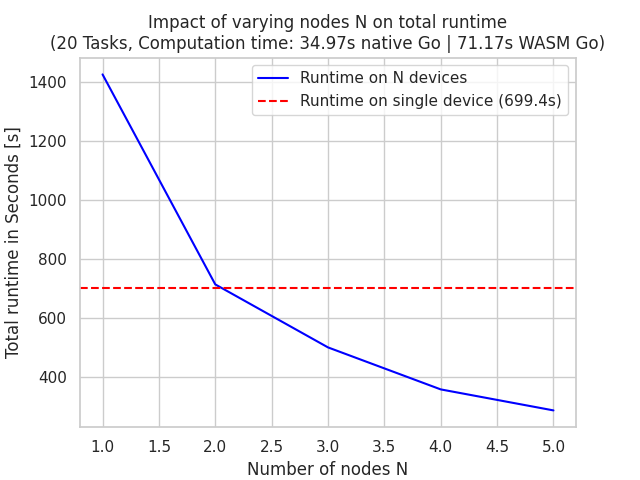
\includegraphics[width=.48\linewidth]{gfx/figures/Theory_A.png}
   } 
   \subfloat[Variable amount of tasks T]{
     \label{fig:background:theoryB}
     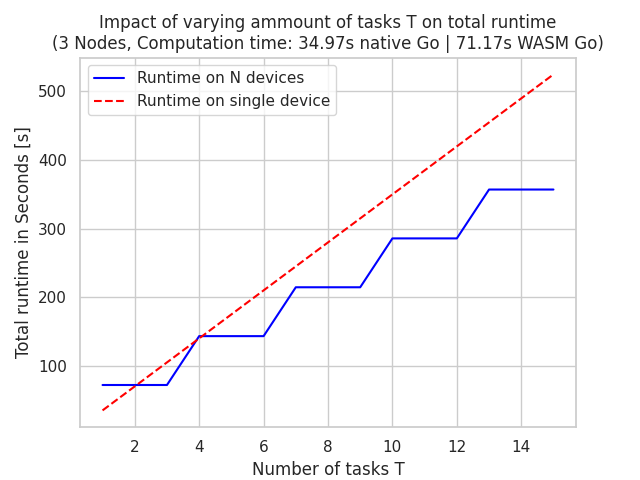
\includegraphics[width=.48\linewidth]{gfx/figures/Theory_B.png}
   }
   \caption{Visualizing the Total Computation Time for an Estimated Example Case}
   \label{fig:background:theoryplot}
\end{figure}
~\\
The graph in \autoref{fig:background:theoryA} represents the total runtime, on the y-axis in seconds, as a function of the number of nodes $N$ in the network, on the x-axis. The red dotted line displays the total execution time $t_{ExSeq}$ on a single machine, while the blue line illustrates the total execution time $t_{ExDist}$ of the volunteer computing network. The total number of all tasks $T$ is set to 20. This plot reveals that the volunteer network achieves a faster total computation time than a single device, if three or more nodes are availabile in the network. The total runtime $t_{ExDist}$ is already by 30\% faster than $t_{ExSeq}$ when the workload is distributed to three nodes.

The other graph in \autoref{fig:background:theoryB} displays the total runtime on the y-axis in seconds as a function of the number of tasks $T$ on the x-axis. The red dotted line represents again $t_{ExSeq}$ of a single device and the blue line $t_{ExDist}$ of the volunteer computing network. The number of nodes $N$ is set to three. This plot demonstrates that the volunteer network achieves faster total computation time than a single device when the workload $T$ consists of more than two tasks. The performance gain grows exponentially as the number of tasks increases. Furthermore, it can be concluded that the total computation time $t_{ExDist}$ of the volunteer network only increases when the number of tasks $T$ and the number of nodes $N$ have no common divisor. However, it is crucial to note that the network will have a longer computation time in every scenario with only one task, as a single task cannot be executed in parallel.

Both plots show, that the total computation time $t_{ExDist}$ is already almost even to the threshold value of $t_{ExSeq}$ if the volunteer network has two participating nodes and faster if there are three or more nodes. This holds true even if the computation time $t_{C}$ of a single task is twice as fast on a native system as measured in the browser environment. This proves that the approach of distributing the workload has a performance gain in this theoretical example, if multiple nodes participate in the volunteer computing network. 

However it needs to be considdered, that if there is only one or two node in the network this approach will already be slower in this example due to the initial offset time, the additional network latency and the higher computation time for each individual task.